\section{Simulation}

\textit{Computational ocean
acoustics} explores algorithms that model
the ocean as an acoustic medium. Works on this matter are well documented by
\citet{Etter2013}. Most of these works focus on very long range simulations,
with its most important features been the ocean floor and sub-bottom region.

This work aims to reconstruct and simulate near-range partially closed
environments, as those created by humans. The motivation for such a choice comes
from the application on hydroeletric power plant water intakes, which is a corridor-like environment
with possible obstacles on the bottom. This kind of environment is not well
covered on the underwater acoustics literature, as such, some of the simulations
techniques are borrowed from the closelly related area of \textit{room
acoustics}.

When constructing a simulation, one has to consider the trade-off between
simplicity, perfomance and accuracy. There are several possible techniques with
different applications and assumptions, this chapter will cover the most
classic ones and further explore \textit{ray theory}, which has been used for
the simulation presented here. For a more comprehensive view on this and other
techniques, see \citet{LURTON,jensen2011computational}.

\subsection{Techniques Overview}
\label{ss:simuloverview}

The idea behind sound simulation techniques is to solve the wave
equation (eq. \ref{eq:wave}) considering all the physical interfaces as boundary
conditions. The equation, however, cannot be analytically solved due to common
present discontinuities caused by occlusions, specular highlights and other
facts that result in large variations of field over small regions of the
domain of integration\cite{funkhouser2003survey}.

The single most important reason that differentiates the several approaches
described here is the \textit{wave frequency}. For high-frequency (where sound
speed do not vary much in a wavelength scale) geometric methods (ray theory) are
justifiable and preferable (in the computational sense) \cite{urick1979}. In the
case of low/mid - frequency or in the presence of caustics\footnote{A region of
high constructive interference that geometrically gives a point of infinity
rays convegence.}, other wave methods (e.g. finite elements, normal modes,
parabolic approximation) should be applied.

%% SrJ: aren't you mjissing a subsubsection here ?

%% SrJ: "assumed" ? Isn't that an analytic solution in case of a sine wave
%% SrJ: (fourier transform and all that)
Instead of using the full wave equation, the methods work with a simplified
time-independent version. As it is a linear equation, it can be assumed that the
equation \ref{eq:wave}:

\[ \nabla^2 p = \frac{1}{c^2_0}\frac{\partial^2}{\partial t^2} p \]

Has a solution where time dependence is a harmonic function:

\begin{equation}
\label{eq:pressurepsi}
p(\coord{x},t) = \Re(\psi(\coord{x})\mathrm{e}^{-i\omega t})
\end{equation}

Here $\coord{x}$ is the space coordinate while $t$ is the time. The exponential
function considered is the complex exponetial with $i$ being the imaginary unit.
The real part $\Re(\parm)$ is taken as $p$ is real-valued, but $\phi(\coord{x})$
is a complex-valued function over space.
%\[ \frac{\partial}{\partial t}\psi = 0 \]
%\[ \nabla^2 \vartheta = 0 \]

Substituting it back into equation \ref{eq:wave}, gives
(dropping explicit parameters again):

\[ \Re(\nabla^2 \psi \mathrm{e}^{-i\omega t}) =
\Re(-(\tfrac{\omega}{c_0})^2 \psi \mathrm{e}^{-i\omega t})\]

% \[ \frac{\nabla^2 \psi}{\psi} = \frac{1}{c_0^2\vartheta} \frac{\partial^2}{\partial
% t^2}\vartheta  \]

Defining $k \equiv \tfrac{\omega}{c_0} $ (a.k.a. the wave number) and rearranging
terms:

\[ \Re((\nabla^2 \psi -k^2 \psi) \mathrm{e}^{-i\omega t}) = 0\]

As the harmonic $\mathrm{e}^{-i\omega t}$ is equivalent to a rotation in the complex
plane, the equation will be satisfied for all $t$ if:

\begin{equation}
\label{eq:helmholtz}
(\nabla^2 -k^2)\psi = 0 
\end{equation}

%  As the expressions on
% both sides vary indepently, ie.
% l.h.s.
% varies with space $x$ and r.h.s. with time $t$, they must be constant. As a matter of ajusting the
% equation to fit its stantard parametrization, this constant is chosen to be
% $-k^2$, then:
% 
% \[ \frac{\nabla^2 \psi}{\psi} = -k^2  \]
% \[ \frac{1}{c_0^2\vartheta} \frac{d^2}{dt^2}\vartheta = -k^2  \]
% 
% Or
% 
% \begin{equation}
% \label{eq:helmholtz}
% (\nabla^2 -k^2)\psi = 0 
% \end{equation}
% 
% \[ (\frac{d^2}{dt^2} + (kc_0)^2)\vartheta = 0  \]
% 
% With the apropriate definition of $\omega \equiv kc_0 $ the last equation,
% becomes:
% 
% \begin{equation}
% (\frac{d^2}{dt^2} + \omega^2)\vartheta = 0
% \end{equation}

Equation \ref{eq:helmholtz} is known as the (homogeneous) \textit{Helmholtz
equation} and describe the time-independent part of the wave propagation. The
values of $k$ and $\omega$ can be phisically interpreted as the spatial and
temporal angular frequency of the wave. As the wave equation is 
linear, superposition applies, being resoanable to take into consideration one
wave frequency at a time and superpose all these harmonics by Fourier synthesis\cite{Lefebvre}.

Fourier synthesis is the calculation by \textit{Helmholtz
equation} of each independent frequency: 

\[ \psi_\omega(\coord{x}) = \int_{-\infty}^\infty p(\coord{x},t)\mathrm{e}^{i\omega t}\dif t \]

And reconstruct the wave equation back by:

\[ p(\coord{x},t) = \int_{-\infty}^\infty\psi_\omega(\coord{x})\mathrm{e}^{-i\omega t}\dif\omega \]

These equations are the inverse and forward Fourier transform, respetively.

\subsubsection{FEM - Finite Element Method}

Finite Element Methods try to numerically find a solution to the wave equation
by discretizing space, and time in some cases. It considers the equation
\ref{eq:wave} for inside the enviroment and the boundary conditions:

\[  \frac{\partial}{\partial \mathbf{n}}p= -\rho_0 \frac{\partial^2
x_n}{\partial t^2} \quad \text{on the source} \]

\[  c_0 \frac{\partial}{\partial \mathbf{n}}p= - \frac{1-R_c}{1+R_c}
\frac{\partial}{\partial t} p \quad \text{on other interfaces} \]

Where $\mathbf{n}$ is the normal direction of the surface, $\rho_0$ is the
medium density and $x_n$ is the displacement of the acoustic membrane. The
reflection coefficient $R_c$ might depend on the interface, but as FEM are used
for small frequency bands, it is a minor problem\cite{deines2006comparative}.

To create a linear system, the pressure function is approximated by a
superposition of functions, e.g. sum of piecewise quadratic functions \(
p(\coord{x},t)= \sum_{i=0}^N p_i(t) \varphi_i(\coord{x}) \), applied to the wave and boundary
equation and integrated w.r.t. $\varphi_i$. Giving a large set of ordinary
differential equations:

\begin{align*}
M\ddot{p} + D\dot{p} + Kp &= Fu \\
y &= Pp
\end{align*}

With \(M,D,K\) being \(N \times N \) matrices, $p$ being the vector with
coeficients $p_i$, $Fu$ the input converted into a force and $P$ some selection
matrix to ouput the pressure on the desired points. This model can be writen and
solved as generalized state-space model:

\begin{align*}
E\dot{\hat{x}} &= A\hat{x} + Bu \\
y &= C\hat{x}
\end{align*}

\[
\hat{x} =
  \begin{bmatrix}
    p \\
    \dot{p}
  \end{bmatrix},~
E =
  \begin{bmatrix}
    I & 0 \\
    0 & M
  \end{bmatrix},~
A =
  \begin{bmatrix}
    0 & I \\
    -K & -D
  \end{bmatrix},~
B =
  \begin{bmatrix}
    0 \\
    F
  \end{bmatrix}
  ~
  \text{and}
  ~
C =
  \begin{bmatrix}
    P & 0 
  \end{bmatrix}
\]
 
 There can be made more simplifications, but it is enough to highlight the
 limitations of the method (For more details, refer to
 \citet{deines2006comparative}). The dimension of the state is related to
 the number of functions used to approximate $N$ (two times without any further
 simplification) that depends on the frequency:
 
 \[N = \left(\frac{nLf}{c_0}\right)^3 \]
 
 Where $L$ is a typical dimension in the environment, $f = \frac{\omega}{2\pi}$
 the frequency and $n$ the number of elements per wave, that should be 3 ou 4
 for a good approximation\cite{deines2006comparative}.
 
 Given that the size of the state increases as the cube of the frequency, the
 technique can only be applied to low-frequency signals, which is not applicable
 to high-frequency sonar as envisoned by this work. 

There is also a boundary method that uses surface integral form of the wave
equation, but suffers from similar restrictions. \citet{funkhouser2003survey}
gives a brief introduction of the subject.

\subsubsection{Ray theory}
\label{sss:raytheory}

Geometric approaches like ray theory dates back to Newton and the corpuscular
theory of light. Later found to be better described as a wave, the geometric
theory of light is still a very important and useful tool. The sound ray theory
%% SrJ: frequency is irrelevant to using geometry, wavelength is. The
% frequencies
%% SrJ: are different, but because of the speeds the wavelengths are not so much
follows a similar path, they both apply to short-wavelength waves, but typical
sound waves have mid-wavelength ($10-10^{-3}$m) while visible light has a
much shortter wavelength ($\approx10^{-6}$m).

To describe the ray from the wave theory, one starts by solving the Helmholtz
equation (eq \ref{eq:helmholtz}) with a generic complex function of space
through a polar decomposition\cite{buckingham1992ocean,torres2007modeling}:

\begin{equation}
\label{eq:psi}
\psi(\coord{x}) = \mathcal{A}(\coord{x})\mathrm{e}^{iw\tau(\coord{x})}
\end{equation}


Here $\tau(\coord{x})$ can be interpreted as the time it takes the sound to
reach the location $\coord{x}$ and $\mathcal{A}(\coord{x})$ the amplitude of the
signal at that point. Substituting it back to equation \ref{eq:helmholtz} and
separating real and imaginary parts, two equations can be obtained (omitting
arguments):

\begin{subequations}
\begin{equation}
\label{eq:preeikonal}
\frac{\nabla^2\mathcal{A}}{\mathcal{A}} - (w\nabla \tau)^2 + k^2 = 0
\end{equation}

\begin{equation}
\label{eq:preeikonalamp}
2(\nabla\mathcal{A} \cdot \nabla \tau) + \mathcal{A}\nabla^2 \tau = 0
\end{equation}
\end{subequations}

The geometric approximation is the assumption that the amplitude does not change
much on the wavelenth scale, mathematically expressed as:

\begin{equation}
\label{eq:highfrequency}
\frac{\nabla^2\mathcal{A}}{\mathcal{A}} \ll k^2
\end{equation}

Applying this approximation to equation \ref{eq:preeikonal} and using the
fact that \(\omega = kc_0 \):

\begin{equation}
\label{eq:eikonal}
\norm{ \nabla \tau } = \frac{1}{c_0}
\end{equation}

The equation \ref{eq:eikonal} is known as the \textit{Eikonal equation} and
defines the surfaces of constant phase. Equation \ref{eq:preeikonalamp}, called
the transport equation, can then be used to find the pressure amplitude of the
wave. However,  when considering intensity, conservation of energy can be used as
will be seen later on subsection \ref{ss:raytheory}.

The rays are, by definition, the perpendicular lines to the wavefronts defined
by equation \ref{eq:eikonal}. Which, with length parametrization, is:

\begin{equation}
\label{eq:ray}
\frac{\dif r}{\dif s} = c_0 \nabla\tau
\end{equation}

Where $r(s)$ is the path follow by the ray, and $s$ the ray length. To verify
that it is a length parametrization square equation \ref{eq:ray} and use
equation \ref{eq:eikonal} to find:

\begin{equation*}
\norm{\frac{\dif r}{\dif s}} = 1 
\end{equation*}

Showing that it is a unit norm tangent vector. To find the ray path, first take
the gradient of equation \ref{eq:eikonal} squared:

\begin{subequations}
\begin{equation}
\nabla(\norm{ \nabla \tau }^2) = \nabla\left(\frac{1}{c_0^2}\right)
\end{equation}
\begin{equation}
2\coord{H}(\tau)\nabla\tau = 2\frac{1}{c_0}\nabla\left(\frac{1}{c_0}\right)
\end{equation}
\begin{equation}
\label{eq:t_hessiantau}
c_0\coord{H}(\tau)\nabla\tau = \nabla\left(\frac{1}{c_0}\right)
\end{equation}
\end{subequations}

The \(\coord{H}(\parm)\) is the Hessian. Also, the derivative of equation
\ref{eq:ray} (divided by $c_0$) w.r.t.
$s$ is:


\begin{subequations}
\begin{equation}
\frac{\dif}{\dif s}\left(\frac{1}{c_0}\frac{\dif r}{\dif s}\right)
=\frac{\dif}{\dif s}(\nabla\tau)
\end{equation}
\begin{equation}
\label{eq:t_dergrad}
\frac{\dif}{\dif s}\left(\frac{1}{c_0}\frac{\dif r}{\dif s}\right)
=\coord{H}(\tau)\frac{\dif r}{\dif s}
\end{equation}
\end{subequations}

Using equation \ref{eq:ray} and \ref{eq:t_hessiantau} in the r.h.s. of equation
\ref{eq:t_dergrad}:

\begin{subequations}
\begin{equation}
\frac{\dif}{\dif s}\left(\frac{1}{c_0}\frac{\dif r}{\dif s}\right)
=\coord{H}(\tau)(c_0\nabla\tau)
\end{equation}
\begin{equation}
\label{eq:raydirection}
\frac{\dif}{\dif s}\left(\frac{1}{c_0}\frac{\dif r}{\dif s}\right)
=\nabla\left(\frac{1}{c_0}\right)
\end{equation}
\end{subequations}

The equation \ref{eq:raydirection} can now be integrated to give the ray path.
Considering the important case of constant sound velocity $c_0$ (as assumed
elsewhere in this work):

\[ \nabla\left(\frac{1}{c_0}\right) = 0 \]

So, equation \ref{eq:raydirection} (with equation \ref{eq:ray}) can be easily
solved to:

\begin{equation}
\label{eq:sray}
r(s) = r_0 + (c_0\nabla\tau_0)s
\end{equation}

Where $r_0$ is the ray origin, $\tau_0$ is the gradient of $\tau$ anywhere
%% SrJ?: "an affine space" OK, either you go all the way or you don't. You can't
%% SrJ: drop something like this at this point, it's ridiculous
%% SrJ: (my advice is "don't", this is engineering, not math, R^3 is an affine
%% SrJ: space)
%% , and the addition is taken with $\mathbb{R}^3$ as an affine space
along the ray.
This is the equation of a line, show that acoustic rays travel as a straight
line on constant velocity mediums for a high-frequency approximation.

Further considerations on reflection and refraction may rely on the
\textit{Snell law} limilar to the electromagnetic case, because the eikonal
equation is equivalent to the \textit{Fermat's principle of least time}. If
the first variation of the time functional is zero:

\begin{equation*}
\delta T[C] = \delta \int \frac{1}{c_0(\coord{x})}
\norm{\coord{x}'} \dif s = 0
\end{equation*}

Here $\coord{x}(s)$ is a parametrization of the path $C$, $x'(s)$ the tangent
vector at $s$ and the whole integral $T[\parm]$ is the time to follow the path
$C$. The \textit{Euler-Lagrange equations} give:


\begin{equation*}
\nabla\left(\frac{1}{c_0}\norm{\coord{x}'}\right) - \frac{\dif}{\dif s}
\nabla'\left(\frac{1}{c_0} \norm{\coord{x}'}\right) = 0
\end{equation*}

Where $\nabla'$ is the gradient taken on the tangent space contaning
$\coord{x}'$.
Which become:

\begin{equation*}
\norm{\coord{x}'}\nabla\left(\frac{1}{c_0}\right) =
\frac{\dif}{\dif s}\left( \frac{1}{c_0}
\frac{\coord{x}'}{\norm{\coord{x}'}}\right)
\end{equation*}

By considering a length parametrization $r$ such that $\norm{r'}=1$, the
result is the same as equation \ref{eq:raydirection}, so all the results follow.

It is important to highlight that this simplification relies only on
the high-frequency assumption \cite{national1969physics}, given at
equation \ref{eq:highfrequency}. A more complete description of the mathematics
envolving the physics behind ray theory can be found at \citet{Lefebvre}.

A important result, commonly applied on algorithms derived from ray theory, is
the summation of energy/intensity of incoherent rays at a point. It starts by
taking the norm of the intensity (equation \ref{eq:intensity_pressure}) and applying the
pressure definition to it (equation \ref{eq:pressurepsi}) to get\footnote{Here
$\mathbb{E}[\parm]$ means the expectation for clarity.}:


\begin{equation}\label{eq:intensity_psi}
I = g_0~\mathbb{E}[\abs{\psi}^2]
\end{equation}

Where $g_0 = \tfrac{1}{\rho c_0}$ (the inverse of the characteristic impedance),
$I$ the intensity and $\phi$ the wave.
For a single ray (equation \ref{eq:psi}) it is:

\begin{equation*}
I = g_0~\mathbb{E}[\abs{\mathcal{A}}^2]
\end{equation*}

To consider the contribution of a set of incoherent rays $\psi_i$ (i.e.
%% SrJ?: I'm not sure about the "statistically" here ... I believe
% "uncorrelated"
%% SrJ: would be enough given the definition of "uncorrelated waves" in physics
uncorrelated), the total $\psi$ becomes:

\begin{equation}\label{eq:wavesum}
\psi = \sum_i \psi_i 
\end{equation}

With the established fact that the expected value of a wave is zero (i.e. the
mean pressure variation is zero), the condition
becomes\footnote{Here $\psi_i^*$ is the complex conjugate of $\psi_i$ for
better reading.}:


\begin{equation}
\label{eq:wave_uncorr}
\text{cov}(\psi_i,\psi_j) = \mathbb{E}[\psi_i \psi_j^*] = 0
\end{equation}

The resulting equation of the intensity (equation \ref{eq:intensity_psi}) for a
full wave (equation \ref{eq:wavesum}) is:

\begin{equation*}
\begin{split}
I &= g_0~\mathbb{E}\left[\abs{ \sum_i \psi_i } ^2\right] =
g_0~\mathbb{E}\left[ (\sum_i \psi_i)(\sum_j \psi_j)^*\right] \\
&= g_0~\mathbb{E}\left[\sum_i \abs{\psi_i}^2 + \sum_{i \neq j} \psi_i
\psi_j^*\right] \\
&= g_0~\mathbb{E}\left[\sum_i \abs{\psi_i}^2\right]  +
g_0~\mathbb{E}\left[\sum_{i \neq j} \psi_i \psi_j^*\right] \\
& = g0~\sum_i \mathbb{E}\left[\abs{\psi_i}^2\right]  + g_0~\sum_{i \neq j}
\mathbb{E}[\psi_i \psi_j^*] \\
& = \sum_i g_0\mathbb{E}\left[\abs{\psi_i}^2\right]
\end{split}
\end{equation*}

Which implies:
\begin{equation}
\label{eq:intensity_sum}
I = \sum_i I_i
\end{equation}

This assumption of incoherent rays will be a common point among ray tracing
algorithm, mainly because it implies the summation of ray intensities $I_i$ to a
single intensity. It is a reasonable assumption on mildly complex environments
with diffuse (scattering) surfaces, which is explained on Ray Theory subsection
\ref{ss:raytheory}.


\subsubsection{Normal modes}

When there is a preferred direction, or a general axis symmetric medium, like the
ocean (which is generally treated as a horizontally stratified medium), a
cylindrical parametrization becomes a useful coordinate system. The principal
axis, in our case depth, contain the superposition of normal modes while the other
dimensions carry the traveling wave.

There are slightly different mathematical approaches to Normal Modes Theory in
the literature\cite{Etter2013,urick1979,buckingham1992ocean}. The following
brief description rely on the techniques of \citet{Etter2013}. Writing the
solution of equation \ref{eq:helmholtz} as a product of a ``depth'' (principal
axis) function $N(z)$ and a horizontal range function $H(r)$:

\[ \psi = N(z)H(r) \]

 Leads to a separation of variables on the ODE, with $k_0$ as separation
 constant: %Yield to
 
 \begin{subequations}
 \begin{equation}
 \label{eq:normalmode}
 \fdif{z}N + (k^2 - k_0^2)N = 0
 \end{equation}
 \begin{equation}
 \label{eq:normaltraveling}
 \fdifn{r}{2}H + \inv{r}\fdif{r}H + k_0^2H = 0
 \end{equation}
 \end{subequations}
 
 The normal mode equation \ref{eq:normalmode} describes the pressure field along
 the depth. Equation \ref{eq:normaltraveling}, on
 the other hand, describes the traveling portion of the wave, that
 happens in the horizontal plane.
 The full solution for $\psi$ is found by solving both equations. The equation
 \ref{eq:normalmode} is a classic eigenvalue problem for the differential
 operator, whose solutions, including boundary conditions, are known as
 Green's function $G$ \cite{desanto2012scalar}. The horizontal equation
 \ref{eq:normaltraveling} is a zero-order Bessel equation, so it may have its
 solution written in terms of the zero order Henkel function of the first kind
 ($H_0^{(1)}$)\footnote{$H_0^{(1)}(x) = J_0(x)+iY(x)$, where $J_0$ and $Y_0$
 are the zero-order Bessel functions of first and second order, respectively.
 More details on these functions, see \citet{abramowitz1964handbook}}. Putting
 these solutions together, for a monochromatic point source:
 
 \begin{equation}
 \label{eq:normalmono}
 \psi(z,r) = \int_{-\infty}^{\infty} G(z,z_s;k_0)H_0^{(1)}(k_0r)k_0\dif k_0
 \end{equation}
 
Where $z_s$ is the source position on the principal axis. The evaluation of the
integral as it appears is impractical, thus some simplifications are required.

The Green's function $G$ can be expanded as a bilinear summation of orthonormal
functions ($u_ n$), the \textit{normal modes}\cite{baker2003green}, weighted by
using their respective eigenvalues ($k_n$), the natural frequencies. The real
integral of equation \ref{eq:normalmono} can be evaluated through \textit{contour
integration} to exploit the residue of the poles present on the natural
frequencies. But this requires to choose a Riemann
sheet for the integral and evaluate the branch line integral
separately\cite{jensen2011computational,worzel1948propagation}:

\begin{equation}
\psi = \oint \sum_n{\frac{u_n(z)\overline{u_n(z_s)}}{k^2 -
k_n^2}H_0^{(1)}(k_0r)k_0\dif k_0} + I_{\text{branch-cut}}
\end{equation}

The branch line integral $I_{\text{branch-cut}}$ can be physically interpreted
%% SrJ: "continuous mode spectrum" ?
as the contribution of all other modes spectrum (those that are not
normal modes), representing modes that propagates through the ocean floor
(being strongly attenuated) and near-field, that decays exponentially with
distance. Assuming that the horizontal distance is several times the water
depth, the branch line term is ignored in most theoretical developments.

Therefore, by assuming a far-field approximation ($k_0r \ll 1$), besides
disregard the branch line integral, it is possible to consider an asymptotic expansion for the
Hankel fucntion and evaluate the contour integral, obtaining\cite{Etter2013}:

\begin{equation}
\label{eq:normalsolution}
\psi =
g(r)\sum_n{\frac{u_n(z)\overline{u_n(z_s)}}{\sqrt{k_n}}\mathrm{e}^{i(k_nr-\tfrac{\pi}{4})-\delta_nr}}
\end{equation}

Here $g(r)$ is a general function of the range and $\delta_n$ the attenuation
coefficient. In practice, the summation ranges over only a bounded number of
modes, but this number increases with frequency, which leaves it as undesirable
for high-frequency waves. 

One of the advantages of normal modes over ray theory lies on the fact that, for
each source/receiver position, the ray approach have to run a full simulation of
the rays, while the normal modes have a closed form (like equation
\ref{eq:normalsolution}) that easily adapts to new combinations of these
parameters. In contrast, normal modes are constrained by the source frequency,
in fact by the number of modes to be computed, and generally requires deeper
knowledge of the environment. The attenuation
coefficient($\delta_n$) in the ocean, for exemple, depends on water absorption,
ocean sediment layer absorptions, compressional and shear attenuation on the
basement, measures of the modes interations with both sediment and
basement(compressional and shear mechanisms) and statistics on the
water-sediment boundary and sea surface as well.

\subsubsection{Parabolic approximation}

The parabolic approximation replaces the Helmholtz equation \ref{eq:helmholtz},
which is a elliptic partial differential equation, by a simplified parabolic
%% SrJ?: give me your time travelling machine ...
version. This approximation dates back to the middle of the $\mathrm{XXI}$
century, in the context of tropospheric radio wave propagation.

The normal mode solution do not handle well non-stratified mediums. To overcome
this limitation parabolic approximation is constructed to handle slow varying
mediums. The variation is made explicit by $k = k_0n(r,z)$, where $n(r,z)$ is a
sound refractive index\cite{LURTON}. The Helmholtz equation becomes:

\begin{equation}
\label{eq:varyhelmholtz}
(\nabla^2 - k_0^2n^2(r,z))\psi = 0 
\end{equation}

The solutions are assumed to have a fast varying horizontal field
$H_0^{(1)}(k_0r)$ and overall slow fluctuations $F(r,z)$:

\begin{equation*}
\psi(r,z) = F(r,z)H_0^{(1)}(k_0r)
\end{equation*}

Assuming asymptotic behavior to the Hankel function (similar to normal modes
development) and applying it to equation \ref{eq:varyhelmholtz}:

\begin{equation}
\label{eq:preparabolic}
\fdifn{r}{2}F + 2ik_0\fdif{r}F + \fdifn{z}{2}F + k_0^2(n^2-1)F = 0
\end{equation}

By the assumption that $F(r,z)$ is a slow varying field, the $\fdifn{r}{2}F$
term is neglected and equation \ref{eq:preparabolic} gives rise to the parabolic
equation. \citet{LURTON} proceeds further by discretizing the horizontal
directions, without defining explicit dependence on the Hankel function, and
using an approximation for the differentials on $z$ through pseudo-differential
operator.

The parabolic equation can then be solved numerically, but the grid size vary
with frequency, becoming costly for high-frequency waves. For more
details, see \citet{jensen2011computational}.

\subsection{Ray Theory}
\label{ss:raytheory}

Ray Theory provides a good way to treat high-frequency sound propagation,
far from caustics, that retain an intuitive meaning. Introduced in subsection
\ref{ss:simuloverview}, it is very similar to its electromagnetic counterpart.
Each ray carries a energy density from the source that decays as it travels
through the medium (Transmission loss). When it encounters an obstacle (e.g. sea floor, sea
surface, man made surfaces), it (back)scatter to the source
(equation~\ref{eq:preeikonalamp)}. That is the
classical (non-multipath) description
\cite{LURTON,Etter2013,miller2015real,bell1997application}, summarized by a
sonar equation as:

\begin{equation}
\label{eq:sonareq}
\text{RL} = \text{SL} - \text{DI} - \text{TL} + \text{TS}
\end{equation}

Each of these acronyms corresponds to energy (intensity), or energy variation,
written in decibels\ref{eq:dB}:
\begin{enumerate}
  \item RL is the Received Level - $10\log_{10}([\text{Received
  intensity}]/[\text{reference intensity\footnotemark}])$
  \footnotetext{Intensity of plane wave with pressure amplitude of 1 $\mu$Pa}
  \item SL is the Source Level - $10\log_{10}([\text{Intensity at
  1m\footnotemark}]/[\text{reference
  intensity}])$
  \footnotetext{for an equivalent omnidirectional source}
  \item DI is the Directivity Index - $10\log_{10}([\text{Directional
  loss\footnotemark}])$
  \footnotetext{with respect to an omnidirectional source}
  \item TL is the Transmission loss - Intensity loss through absorption and
  spreading while propagating (in dB).
  %% SrJ: I don't get the difference between TS and RL
  \item TS is the Target Strength - ratio between the intensity of outgoing
  and incoming rays on a target hit (in dB).
\end{enumerate}



Equation (\ref{eq:sonareq}) does not fully describes how the simulation
using ray theory should work, but gives a good insight on the elements that must
be considered. SL can be inferred by the sonar power and efficiency, DI comes
from the sonar beam pattern, TL is dependent on the medium, but is compensated
by the sonar TVG (see subsection \ref{sss:tvg}) and TS is defined by a material
dependent BRDF (Bidirectional Reflectance Distribution Function), described further ahead.

\subsubsection{Ray Interaction}

For a more faithful sonar response, advanced simulation techniques based on ray
theory can be applied. And, thus, requires careful consideration on the most
important interactions of the rays with the interfaces, namely:
\textbf{transmitted rays}, \textbf{reflected rays}  and \textbf{scattered rays},
see figure \ref{fig:brdfbtdf}.

\subsubsection{Transmitted Rays}
When a radiant energy, in this setup represented by a ray, hits a point on a
surface (or a general interface) part of the energy is absorbed, part is
transmitted and, yet, another part bounces back Transmitted rays represent the
energy that goes through the interface, their intensity for each direction is
%% BDTF -> "Transmitted Scatter" ?
mathematically defined by the BTDF (Transmitted Scatter Distribution
Function)\cite{bartell1981theory} (see \citet{rober2007ray} for a acoustic
approach).


\begin{figure}[h]
	\centering
	\begin{tikzpicture}[line cap=round,line join=round,>=triangle 45,x=1.0cm,y=1.0cm]
\clip(-4.78,-2.94) rectangle (4.8,3.36);
%\draw [shift={(0.,-2.)},color=qqwuqq,fill=qqwuqq,fill
% opacity=0.10000000149011612] (0,0) -- (90.:0.6) arc (90.:123.69006752597979:0.6) -- cycle;

%\draw [shift={(0.,-2.)},color=qqwuqq,fill=qqwuqq,fill
% opacity=0.10000000149011612] (0,0) -- (23.19859051364819:0.6) arc (23.19859051364819:90.:0.6) -- cycle;

\draw [line width=2.8pt] (-3.,-2.)-- (3.,-2.);
\draw [dash pattern=on 1pt off 1pt] (0.,-2.)-- (0.,2.);
\draw (0.,-2.)-- (7.,1.);
\draw (3.596510228151898,-0.4586384736491866) -- (3.55317910530819,-0.6240845790524369);
\draw (3.596510228151898,-0.4586384736491866) -- (3.446820894691815,-0.3759154209475615);

\draw [shift={(0.,-2.)},->,color=qqwuqq] (90.:0.6) arc (90.:123.:0.6);

\draw [shift={(0.,-2.)},<-,color=qqwuqq] (23.2:0.6) arc
(23.2:90.:0.6);

\draw (-4.,4.)-- (0.,-2.);
\draw (-1.9417564793963522,0.9126347190945269) -- (-2.11232678973561,0.9251154735095947);
\draw (-1.9417564793963522,0.9126347190945269) -- (-1.8876732102643923,1.0748845264904066);
\begin{scriptsize}
\draw[color=black] (3.93,-0.56) node {$I_r$};
\draw[color=qqwuqq] (-0.35,-0.42) node {$\theta_i$};
\draw[color=qqwuqq] (0.95,-0.92) node {$\theta_r$};
\draw[color=black] (-2.37,1.06) node {$I_i$};
\end{scriptsize}
\end{tikzpicture}
	\caption{Incident and reflected rays with respective angles.}
	\label{fig:ray_reflect}
\end{figure}


\subsubsection{Scattered and Reflected rays}
\label{sss:rays}
The treatment for reflected and scattered rays starts together by means of the
BRDF (Bidirectional Reflectance Distribution
Function)\cite{blake1995remote,miller2015real,durany2015analytical}, which works
similar to BTDF. On perfect smooth surfaces, its BRDF exhibits a single
direction, the specular reflection, where the ray intensity is non-zero at the
same plane of incident ray and the same angle with the surface normal vector.
This kind of reflection is responsible for mirror like effects, e.g. sound that hits
the still water surface from within\cite{LURTON,Etter2013}.

The other extreme case is the perfect diffuse reflection (usually called scatter
in acoustics), where a rough surface reflects same perceived energy (radiance)
in all directions, thus following a cosine law (Lambert's Cosine Law) with
respect to the incident and reflected(scattered) angles
\cite{united1977geometrical,cox2004acoustic}:

\begin{equation}
\label{eq:lambertian}
I_r \propto	 I_i \cos(\theta_i) \cos(\theta_r)
\end{equation}

Where $I_i$,  $I_r$ and $\theta_i$, $\theta_r$ are the intensity and angle with
the surface normal for the incident and reflected rays,
respetively (figure \ref{fig:ray_reflect}). The proportionality constant is
material dependent and should not exceed $\nicefrac{1}{\pi}$, because that would violate
energy conservation.

If incoming and reflected rays have the same direction, the angle is the same
and the situation is called a \textit{backscatter}:

\begin{equation*}
I_r \propto I_i \cos^2(\theta_i)
\end{equation*}

There is some confusion in the literature about the cosine being or not
squared\cite{durany2015analytical,cox2006tutorial,cox2004acoustic,jones2009modelling,LURTON,Etter2013}.
Possible explanations are mixing intensity information with pressure
or related quantities, as intensity and radiance. This cosine law, for a single
scatter, describes the Target Strength, in $\text{dB}$:

\begin{equation*}
\text{TS} = A + 20\log_{10}(\cos(\theta_i))
\end{equation*}

Here $A$ is the equivalent of the proportionality constant. Under the assumption
of no energy loss through transmission or absorption,
$A=-10\log_{10}(\pi)\text{dB} \approx -5\text{dB}$. More realistic values vary
from $-17\text{dB}$ for basalt ridge cliffs to $-27\text{dB}$ for sediment
pond\cite{dunn2015springer}.
Transmission and reflection between mutiple sedment layers at the bottom of the
ocean can be treated as a single entity, subbottom scattering, that introduces a
delay and a displacement of the reflection\cite{Etter2013}, that case will not
be covered by the simulation procedure proposed in this thesis. A remarkable
property of the scattered rays is the incoherence which makes possible to add
the energy (intensity) contributions for each ray directly, according to
equation \ref{eq:intensity_sum}.

Rough ocean surface, in the presence of wind, also backscatters, but not as a
perfect scatter. Its scattering properties have been modeled in a variety of
ways\cite{jones2009modelling}, like Kirchhoff model\cite{dunn2015springer}:

\begin{equation*}
\text{TS} = -10~\Gamma^2\log_{10}(e) \approx -4.34~\Gamma^2
\end{equation*}

Where $\Gamma = 2kh\cos(\theta_i)$, $k$ is the acoustic wavenumber (equation
\ref{eq:helmholtz}), $h$ is the rms height of the surface.

A general surface does not follow neither a perfect cosine law nor is a perfect
reflector, but is useful to model as a compromise of
both\cite{cox2006tutorial,vorlander2000definition}, even some standards for
acoustic measurement (e.g. ISO) split between these two types of
reflection\cite{rindel2001scattering}. A absorption/transmission factor $\alpha$
defines the fraction of the energy that does not reflect back, and a scattering
factor $\delta$ the fraction of the reflected energy that is scattering (figure
\ref{fig:scatter}).

\begin{figure}[h]
	\centering
	\begin{tikzpicture}[line cap=round,scale = 2,line join=round,>=triangle
45,x=1.0cm,y=1.0cm] \clip(2.7948180794505695,-1.3697087422553846) rectangle
(8.79508118638861,1.4018876685668866); \draw [line width=2.4pt] (0.32,-1.1)--
(0.4,-1.1)-- (0.5,-1.06)-- (0.56,-1.04)-- (0.72,-1.02)-- (0.8,-1.)--
(0.9,-0.98)-- (1.04,-0.96)-- (1.14,-0.96)-- (1.24,-0.96)-- (1.34,-0.96)--
(1.44,-0.96)-- (1.6,-0.96)-- (1.68,-0.96)-- (1.76,-0.96)-- (1.86,-0.96)--
(1.98,-0.96)-- (2.06,-0.96)-- (2.18,-0.96)-- (2.26,-0.96)-- (2.32,-0.98)--
(2.4,-1.)-- (2.46,-1.02)-- (2.52,-1.04)-- (2.66,-1.06)-- (2.76,-1.06)--
(2.84,-1.06)-- (2.94,-1.08)-- (3.04,-1.08)-- (3.14,-1.08)-- (3.22,-1.08)--
(3.28,-1.06)-- (3.36,-1.04)-- (3.48,-1.02)-- (3.56,-1.02)-- (3.64,-1.02)--
(3.74,-1.02)-- (3.86,-1.02)-- (3.92,-0.98)-- (4.02,-0.92)-- (4.1,-0.86)--
(4.16,-0.82)-- (4.22,-0.78)-- (4.3,-0.76)-- (4.38,-0.76)-- (4.44,-0.78)--
(4.52,-0.8)-- (4.58,-0.86)-- (4.64,-0.9)-- (4.72,-0.92)-- (4.82,-0.86)--
(4.92,-0.76)-- (4.98,-0.7)-- (5.04,-0.68)-- (5.12,-0.68)-- (5.2,-0.72)--
(5.26,-0.76)-- (5.32,-0.78)-- (5.4,-0.76)-- (5.48,-0.74)-- (5.56,-0.74)--
(5.62,-0.76)-- (5.7,-0.78)-- (5.78,-0.8)-- (5.84,-0.82)-- (5.94,-0.82)--
(6.04,-0.82)-- (6.14,-0.8)-- (6.24,-0.8)-- (6.32,-0.8)-- (6.4,-0.8)--
(6.48,-0.8)-- (6.54,-0.82)-- (6.6,-0.84)-- (6.66,-0.86)-- (6.76,-0.86)--
(6.82,-0.84)-- (6.88,-0.82)-- (6.96,-0.8)-- (7.06,-0.8)-- (7.14,-0.8)--
(7.2,-0.82)-- (7.3,-0.82)-- (7.42,-0.78)-- (7.48,-0.76)-- (7.56,-0.78)--
(7.64,-0.78)-- (7.72,-0.78)-- (7.78,-0.8)-- (7.86,-0.8)-- (7.94,-0.84)--
(8.02,-0.86)-- (8.14,-0.86)-- (8.22,-0.86)-- (8.28,-0.88)-- (8.36,-0.88)--
(8.44,-0.88)-- (8.54,-0.9)-- (8.6,-0.92)-- (8.66,-0.94)-- (8.74,-0.94)--
(8.8,-0.92)-- (8.86,-0.86)-- (8.92,-0.82)-- (8.98,-0.78)-- (9.06,-0.78)--
(9.16,-0.8)-- (9.22,-0.84)-- (9.28,-0.86)-- (9.38,-0.86)-- (9.44,-0.84)--
(9.54,-0.86)-- (9.62,-0.88)-- (9.7,-0.92)-- (9.8,-0.92)-- (9.9,-0.92)--
(10.,-0.92)-- (10.08,-0.92)-- (10.16,-0.92); \draw(5.4,0.02) circle
(0.7777040114412194cm); \draw [line width=1.2pt] (3.2,1.22)--
(5.409411764705884,-0.7576470588235291); \draw [line width=1.2pt]
(4.348182392416691,0.19226059549922564) --
(4.25606103849168,0.1768308330085503); \draw [line width=1.2pt]
(4.348182392416691,0.19226059549922564) --
(4.353350726214204,0.28552210816792145); \draw [line width=1.2pt,]
(5.409411764705884,-0.7576470588235291)-- (8.,0.86); \draw [line width=1.2pt,]
(6.754198696011041,0.08208138374894797) --
(6.743337023803831,-0.010689546484390354); \draw [line width=1.2pt,]
(6.754198696011041,0.08208138374894797) --
(6.666074740902051,0.1130424876608616); \draw [->,line width=0.4pt]
(5.409411764705884,-0.7576470588235291) --
(5.935960678382477,0.2348997061154039); \draw [->,line width=0.4pt]
(5.409411764705884,-0.7576470588235291) --
(5.401091195592214,-0.13464648199423213); \draw [->,line width=0.4pt]
(5.409411764705884,-0.7576470588235291) --
(4.924571110924526,0.020951912999298772); \draw [->,line width=0.4pt]
(5.409411764705884,-0.7576470588235291) --
(5.109344204979343,0.32242380329926523); 

\draw [->,line width=0.4pt]
(5.409411764705884,-0.7576470588235291) --
(5.744213687769606,0.390498101108935); 

\draw [->,line width=0.4pt]
(5.409411764705884,-0.7576470588235291) --
(5.994310076505051,-0.12492158230713646); \draw [->,line width=0.4pt]
(5.409411764705884,-0.7576470588235291) --
(4.898642259658603,-0.5745283387791806); \draw [->,line width=0.4pt]
(5.409411764705884,-0.7576470588235291) --
(4.817597214366473,0.38077320142183924); \draw [->,line width=0.4pt]
(5.409411764705884,-0.7576470588235291) --
(5.27466749965997,0.6044458942250401); \draw [->,line width=0.4pt]
(5.409411764705884,-0.7576470588235291) --
(5.801414628271618,-0.6461004621086246); \draw
(2.3671152706892486,0.886467985150815) node[text
width=3cm,align=center,anchor=north west] {Incident \\ $1$}; \draw
(4.875946612489047,1.4310623676281735) node[text width=2cm,align=center,anchor=north west] {Scattered
\((1-\alpha)\delta\)}; \draw (7.3308442270661695,0.5363715964153702)
node[text width=3cm,align=center,anchor=north west]
{Specular \\ \((1-\alpha)(1-\delta)\)}; \draw
(4.798147414992282,-1.0974115510167053) node[anchor=north west] {\textbf{Rough Surface}};
\end{tikzpicture}
	\caption{Scattering reflection weighted.}
	\label{fig:scatter}
\end{figure}

This weighting concept is explored to create a full BRDF function as
$\rho(\vec{i},\vec{r}) = (1-\alpha)(\delta \rho_\text{scat}(\vec{i},\vec{r}) +
(1-\delta) \rho_\text{spec}(\vec{i},\vec{r}) )$. For a numerical treatment, one
option is to discretize the solid angles as \citet{siltanen2007room} describes,
another is to model as computer graphics, where, instead of a single direction
for the specular reflection, the specular reflection is a smooth function of the
reflected direction with a peak at the actual specular direction. This smooth
fucntion creates a better transition from specular to scatter reflection. A
standard model is Phong reflection\cite{phong1975illumination}:

\begin{equation}
\label{eq:phong}
I_r \propto	 I_i \cos(\theta_s)^\nu
\end{equation} 

Here $\theta_s$ is the angle between the reflected direction and the specular
direction. And $\nu$ a shininess constant describing how concetrated the
specular reflection is. In the limit of $\nu \to \infty$ it becomes a perfect mirror.


\begin{figure}
	\centering
	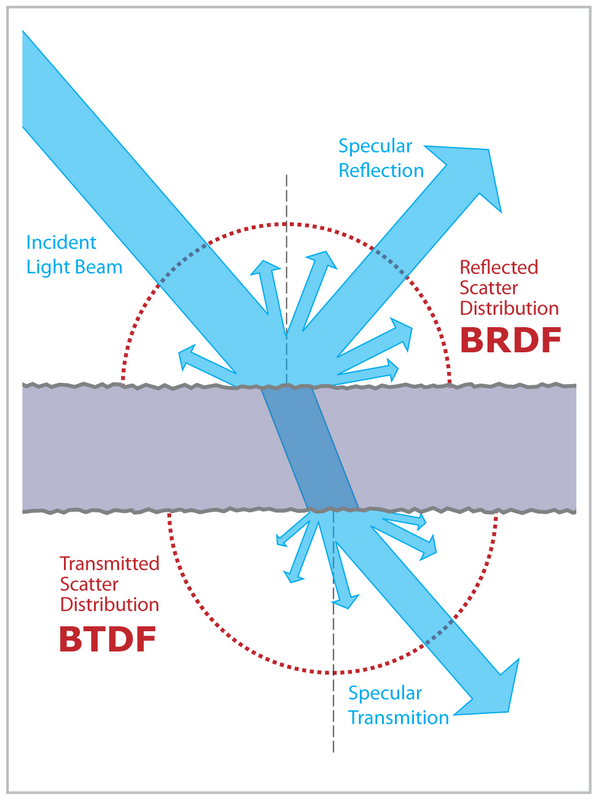
\includegraphics[width=0.8\textwidth]{Chap2/fig/BRDF_BTDF}
	\caption{BRDF and BTDF for transmitted, reflected and scattered rays.
	(\textcopyright  \href{http://commons.wikimedia.org/wiki/User:Jurohi}{User:Jurohi} /
	\href{http://commons.wikimedia.org/}{Wikimedia Commons} /
	\href{http://creativecommons.org/licenses/by-sa/3.0/}{CC-BY-SA-3.0})}
	\label{fig:brdfbtdf}
\end{figure}




\subsubsection{Ray Tracing}

Ray Tracing was originally an algorithm that used ray theory
(described earlier in section \ref{sss:raytheory}) for computer graphics with a
rationale very similiar to the sonar equation \ref{eq:sonareq}. It traced a ray to every point on the scene
from the source and the receiver, then computed the intensity of each color,
ignoring multiple reflections. 

A variety of derivations from the original algorithm have being concieved. Most
of the methods applied to audio were developped for computer graphics
%% SrJ: "rederization" ? Is that "rendering" ?
rendering, but, considering sound waves with similar constrains to those
applyed to light (i.e. high frequency limit), it is reasonable to apply them to
aurelization (sound renderization) as well.


Among the most commum techniques are \textbf{Image Source}, \textbf{Beam
Tracing}, \textbf{Metropolis Transport} and \textbf{Path Tracing}. Their
standard implementation assume homogeneos medium, effectively propagating rays
as straight lines. An important altenative, which also overcome sharp shadows
and caustics issues, is \textit{Gaussian Beam}, it evaluates the acoustic field
at every point by adding contributions of each ray. The name comes from the fact
that weight of a ray decays in the paraxial direction as a gaussian. It is
typically more computationally more costly than other ray tracing, but have
applications for inhomogeneos open environments as described by
\citet{traceroutdoor}.

\subsubsection{Image Source}

This method focus on environments composed by segments on the 2D case or
polygonal slices of planes on the 3D case. It works best on box like
environments, for this creates a perfect tiling of
space\cite{funkhouser2003survey} (see figure \ref{fig:tillingsource}).

For each reflective surface, a virtual source is created on the reflected
position of the source, these are the primary virtual sources. A virtual source
will act just like a source, although its intensity is lessened by the absorption
factor of the wall. When computing the sound at point, the
contribution of each source (including virtual ones) are added together, the
reflections are automatically taken into account by the virtual sources.

\begin{figure}[h]
	\centering
	\begin{tikzpicture}[line cap=round,line join=round,>=triangle 45,x=1.0cm,y=1.0cm]
\clip(-0.738945892060669,-4.142976374738391) rectangle (10.544316672135889,6.890164605522789);
\fill[color=zzttqq,fill=zzttqq,fill opacity=0.03999999910593033] (6.98,-1.7) -- (2.5,0.24) -- (1.42,2.14) -- (8.58,4.08) -- cycle;
\draw [line width=3.6pt,color=zzttqq] (6.98,-1.7)-- (2.5,0.24);
\draw [line width=3.6pt,color=zzttqq] (2.5,0.24)-- (1.42,2.14);
\draw [line width=3.6pt,color=zzttqq] (1.42,2.14)-- (8.58,4.08);
\draw [line width=3.6pt,color=zzttqq] (8.58,4.08)-- (6.98,-1.7);
\draw [dotted,domain=2.5:10.544316672135889] plot(\x,{(--2.78629146637635-1.0568461602880828*\x)/0.6007336069005946});
\draw [dash pattern=on 2pt off 2pt] (5.708632716051649,0.1368818392672047)-- (0.9470693465169548,-2.5696910234156736);
\draw [dash pattern=on 2pt off 2pt] (5.708632716051649,0.1368818392672047)-- (4.770494801176167,-2.029539737352464);
\draw [dash pattern=on 2pt off 2pt] (5.708632716051649,0.1368818392672047)-- (4.110760655764572,6.034182845275178);
\draw [dash pattern=on 2pt off 2pt] (5.708632716051649,0.1368818392672047)-- (9.014969946431826,-0.7783672210456472);
\draw [color=ffqqqq] (5.708632716051649,0.1368818392672047)-- (7.633155810755908,0.6595253663557199)-- (6.96,1.36);
\draw [dash pattern=on 2pt off 2pt] (9.014969946431826,-0.7783672210456472)-- (7.633155810755908,0.6595253663557199);
\begin{scriptsize}
\draw [fill=qqqqff] (5.708632716051649,0.1368818392672047) circle (2.5pt);
\draw[color=qqqqff] (5.903171725779176,0.651020650689955) node {$E$};
\draw [fill=qqqqff] (4.770494801176167,-2.029539737352464) circle (2.5pt);
\draw[color=qqqqff] (5.041641825557272,-1.5166997434167757) node {$E'$};
\draw [fill=qqqqff] (9.014969946431826,-0.7783672210456472) circle (2.5pt);
\draw[color=qqqqff] (9.363186970218761,-0.19661360597998456) node {$E'_1$};
\draw [fill=qqqqff] (4.110760655764572,6.034182845275178) circle (2.5pt);
\draw[color=qqqqff] (4.471920439926657,6.612251734483465) node {$E'_2$};
\draw [fill=qqqqff] (0.9470693465169548,-2.5696910234156736) circle (2.5pt);
\draw[color=qqqqff] (1.303713710078363,-1.9752559806316612) node {$E'_3$};
\draw [fill=ffqqqq] (6.96,1.36) circle (2.5pt);
\draw[color=ffqqqq] (7.153779645456134,1.8738372832629824) node {$R$};
\end{scriptsize}
\end{tikzpicture}
	\caption{The source E and the virtual sources E',E'$_1$,E'$_2$,E'$_3$. In this
	case, E'$_3$ is not a visible virtual source.}
	\label{fig:imagesource}
\end{figure}


The procedure of creating the virtual sources may be repeated many times for
each new virtual sources, thus more reflection are effectivelly calculated. The
visibility of a virtual source must be validated before adding its contribution.

\begin{figure}[h]
	\centering
	\begin{tikzpicture}[line cap=round, scale = 0.4, line join=round,>=triangle
45,x=1.0cm,y=1.0cm] \clip(-9.474877628501186,-5.530684966626176) rectangle (10.523163475369893,5.795406644107648);
\fill[color=zzttqq,fill=zzttqq,fill opacity=0.10000000149011612] (-2.,-1.) -- (-2.,4.) -- (1.,4.) -- (1.,-1.) -- cycle;
\draw [color=zzttqq] (-2.,-1.)-- (-2.,4.);
\draw [color=zzttqq] (-2.,4.)-- (1.,4.);
\draw [color=zzttqq] (1.,4.)-- (1.,-1.);
\draw [color=zzttqq] (1.,-1.)-- (-2.,-1.);
\draw [domain=1.0:10.523163475369893] plot(\x,{(--12.-0.*\x)/3.});
\draw [domain=1.0:10.523163475369893] plot(\x,{(-3.-0.*\x)/3.});
\draw [domain=-9.474877628501186:-2.0] plot(\x,{(-12.-0.*\x)/-3.});
\draw [domain=-9.474877628501186:-2.0] plot(\x,{(--3.-0.*\x)/-3.});
\draw (-2.,-1.) -- (-2.,-5.530684966626176);
\draw (1.,-1.) -- (1.,-5.530684966626176);
\draw (1.,4.) -- (1.,5.795406644107648);
\draw (-2.,4.) -- (-2.,5.795406644107648);
\draw [domain=-9.474877628501186:10.523163475369893] plot(\x,{(--27.-0.*\x)/3.});
\draw (4.,-5.530684966626176) -- (4.,5.795406644107648);
\draw [domain=-9.474877628501186:10.523163475369893] plot(\x,{(-18.-0.*\x)/3.});
\draw (-5.,-5.530684966626176) -- (-5.,5.795406644107648);
\draw (-8.,-5.530684966626176) -- (-8.,5.795406644107648);
\draw (7.,-5.530684966626176) -- (7.,5.795406644107648);
\draw (10.,-5.530684966626176) -- (10.,5.795406644107648);
\begin{scriptsize}
\draw [fill=ubqqys] (-1.06,2.82) circle (2.5pt);
\draw[color=ubqqys] (-0.9737392617439009,3.0689982807349465) node {E};
\draw [fill=qqqqff] (3.06,2.82) circle (2.5pt);
\draw [fill=qqqqff] (-2.94,2.82) circle (2.5pt);
\draw [fill=qqqqff] (-1.06,5.18) circle (2.5pt);
\draw [fill=qqqqff] (-1.06,-4.82) circle (2.5pt);
\draw [fill=qqqqff] (-2.94,-4.82) circle (2.5pt);
\draw [fill=qqqqff] (-2.94,5.18) circle (2.5pt);
\draw [fill=qqqqff] (3.06,5.18) circle (2.5pt);
\draw [fill=qqqqff] (3.06,-4.82) circle (2.5pt);
\draw [fill=qqqqff] (4.94,-4.82) circle (2.5pt);
\draw [fill=qqqqff] (4.94,2.82) circle (2.5pt);
\draw [fill=qqqqff] (4.94,5.18) circle (2.5pt);
\draw [fill=qqqqff] (-7.06,2.82) circle (2.5pt);
\draw [fill=qqqqff] (-7.06,5.18) circle (2.5pt);
\draw [fill=qqqqff] (-7.06,-4.82) circle (2.5pt);
\draw [fill=qqqqff] (-8.94,2.82) circle (2.5pt);
\draw [fill=qqqqff] (-8.94,5.18) circle (2.5pt);
\draw [fill=qqqqff] (9.06,5.18) circle (2.5pt);
\draw [fill=qqqqff] (9.06,2.82) circle (2.5pt);
\draw [fill=qqqqff] (9.06,-4.82) circle (2.5pt);
\end{scriptsize}
\end{tikzpicture}
	\caption{Source on a perfect tilling. The simple pattern facilites
	computation.}
	\label{fig:tillingsource}
\end{figure}

The method does not direct implement the ideia of sound scattering, but there
are some possible extensions\cite{chandak2011fast}. In practice, for more
complex environments, only a few early reflection are generated. The number
$O(n^r)$ of sources, where $n$ is the number of surface planes and $r$ the
number of reflections, that must be created and validated grows exponentially
fast.

\subsubsection{Beam Tracing}

Beam Trancing uses pyramidals beams, a colection of rays, instead of single
infinitesimal rays to calculate reflections \cite{funkhouser2003survey}. The
solid angle on the source that decribes avaiable sound directions can be
subdivided in pyramidal beams without overlap, avoiding sampling issues. These
pyramidal beams exploit the spacial relation between neaby rays, being able to
consider the propagation path witout skiping any ray.

\begin{figure}[h]
	\centering
	\begin{tikzpicture}[line cap=round, scale = 0.8, line join=round,>=triangle
45,x=1.0cm,y=1.0cm] \clip(-5.512273934131843,-0.9049832635138173) rectangle (6.493399860001415,6.090327768635652);
\fill[color=wqwqwq,fill=wqwqwq,fill opacity=0.05] (0.92,0.08) -- (-1.28,1.46) --
(-1.74,3.36) -- (-1.16,5.38) -- (1.26,5.78) -- (4.9,2.16) -- (4.52,-0.3) -- cycle; 
\fill[color=ffqqqq,fill=ffqqqq,fill opacity=0.1] (-1.74,3.36) --
(0.023050081907792185,5.575545468083932) -- (1.26,5.78) -- (3.704588716713291,3.3488430894224965) -- (-1.28,1.46) -- cycle; 
\fill[color=ffqqqq,fill=ffqqqq,fill opacity=0.10000000149011612] (1.72,1.8) -- (-1.28,1.46) -- (0.7597610405323656,2.2329401088929215) -- cycle;
\draw [color=wqwqwq] (0.92,0.08)-- (-1.28,1.46);
\draw [color=wqwqwq] (-1.28,1.46)-- (-1.74,3.36);
\draw [color=wqwqwq] (-1.74,3.36)-- (-1.16,5.38);
\draw [color=wqwqwq] (-1.16,5.38)-- (1.26,5.78);
\draw [color=wqwqwq] (1.26,5.78)-- (4.9,2.16);
\draw [color=wqwqwq] (4.9,2.16)-- (4.52,-0.3);
\draw [color=wqwqwq] (4.52,-0.3)-- (0.92,0.08);
\draw [dash pattern=on 2pt off 2pt,domain=-1.28:6.493399860001415] plot(\x,{(-1.6161260623822482-1.744285116181704*\x)/0.4223006070755704});
\draw [color=ffqqqq] (-1.74,3.36)-- (0.023050081907792185,5.575545468083932);
\draw [color=ffqqqq] (0.023050081907792185,5.575545468083932)-- (1.26,5.78);
\draw [color=ffqqqq] (1.26,5.78)-- (3.704588716713291,3.3488430894224965);
\draw [color=ffqqqq] (3.704588716713291,3.3488430894224965)-- (-1.28,1.46);
\draw [color=ffqqqq] (-1.28,1.46)-- (-1.74,3.36);
\draw [color=ffqqqq] (1.72,1.8)-- (-1.28,1.46);
\draw [color=ffqqqq] (-1.28,1.46)-- (0.7597610405323656,2.2329401088929215);
\draw [color=ffqqqq] (0.7597610405323656,2.2329401088929215)-- (1.72,1.8);
\draw [dotted] (-4.103299141720746,0.390148628846557)-- (-1.74,3.36);
\draw [dotted] (-4.103299141720746,0.390148628846557)-- (-1.28,1.46);
\draw [dotted] (-4.103299141720746,0.390148628846557)-- (1.72,1.8);
\begin{scriptsize}
\draw [fill=qqqqff] (1.72,1.8) circle (2.5pt);
\draw[color=qqqqff] (1.908451589835734,2.2872059376022698) node {$S$};
\draw [fill=qqqqff] (-4.103299141720746,0.390148628846557) circle (2.5pt);
\draw[color=qqqqff] (-4.3991651055367065,0.8825686062798352) node {$S'$};
\end{scriptsize}
\end{tikzpicture}
	\caption{A 2D view of a piramidal beam tracing.}
	\label{fig:beamtrace}
\end{figure}

The algorithm starts by subdividing the sounce sound directions into pyramidal
regions. For each pyramidal beam, intersections with enviroment walls are
calculated from the first encounter to the last, cliping the beam so no
shadowed regions are considered. The resulting polygons of each intersection act
as a new virtual source, constructed by mirroring the source as in the Image
Source method. Beam Tracing, then, progresses by repeating this procedure on
each virtual source, until the desired precision (number of reflections) is
archieved.

It does no suffer from visibility computation issued as Image Source, but is
less efficient for highly structured box-like environments. Despite working well
on simple scenes (with or without occlusions), it still not handeling well
curved surfaces.


\subsubsection{Path Tracing}

Path Tracing is a recursive solution to the wave equation simplification used in
ray theory. That can be written, in terms of the radiance $\ell$ (the ray
energy - acoustic energy per unit of surface area per unit of solid angle), as an
integral equation, the \textit{room acoustics rendering
equation}\cite{siltanen2007room}:

\begin{equation}
\label{eq:roomacoustics}
\ell (\coord{p},\Omega) = \ell_0(\coord{p},\Omega) + \int_\mathcal{G}
R(\coord{x},\coord{p},\Omega) \ell
(\coord{x},\overrightarrow{\coord{x}\coord{p}} ) \dif\mu(\coord{x})
\end{equation}

Where $\mathcal{G}$ is the two dimensional subset of $\mathbb{R}^3$ comprising
all surfaces, $\coord{p}$ is a point over a surface, $\dif\mu(\coord{x})$ is the
surface area differential at point $\coord{x}$, $\Omega$ is the outgoint
%% SrJ: I don't understand the "source point" comment ... It's surface radiance
%% SrJ: ... so I would write e.g. "in case the surface is an emitter", no?
energy direction, $\ell_0$ the intrinsic surface radiance (in case the surface is an emitter), $\overrightarrow{\coord{x}\coord{p}}$ the unit vector in the direction to $\coord{p}$ from point $\coord{x}$. The function $R(\parm,\parm,\parm)$ is the
\textit{reflection kernel}, an enhanced version of a BDRF. For a non-obstructed path between 
$\coord{p}$ and $\coord{x}$:

\begin{equation}
\label{eq:reflectionkernel}
R(\coord{x},\coord{p},\Omega) =
\mathfrak{a}(\norm{\coord{p}-\coord{x}})\rho_\coord{p}(\overrightarrow{\coord{x}\coord{p}},\Omega)\cos(\theta_i)\cos(\theta_r)
\end{equation}

When there is no visibility from  $\coord{x}$ to $\coord{p}$,
$R(\coord{p},\coord{x},\Omega) = 0$. Here
$\rho_\coord{p}(\overrightarrow{\coord{x}\coord{p}},\Omega)$ is the BDRF at the
point $\coord{p}$ with incoming direction $\overrightarrow{\coord{x}\coord{p}}$
%% SrJ?: omega is not a direction, but the incoming energy, or ?
and outgoing direction $\Omega$, $\theta_i$ and $\theta_r$ are the incoming and
reflected angles with surface's normal at point $\coord{p}$ for directions $\overrightarrow{\coord{x}\coord{p}}$
and $\Omega$ respectively. Factor $\mathfrak{a}(\norm{\coord{p}-\coord{x}})$ is
the decay dependent on the distance $\norm{\coord{p}-\coord{x}}$ caused
by spreading and absoption, usually a inverse squared times a exponential factor (commented on subsection \ref{sss:tvg}).

The solution to equation \ref{eq:roomacoustics} is a Neumann series:



\begin{subequations}

\begin{equation}
\label{eq:neumannincrement}
\ell_{n+1} (\coord{p},\Omega) = \int_\mathcal{G}
R(\coord{x},\coord{p},\Omega) \ell_n
(\coord{x},\overrightarrow{\coord{x}\coord{p}} ) \dif\mu(\coord{x})
\end{equation}

\begin{equation}
\label{eq:neumannsummation}
\ell (\coord{p},\Omega) = \sum_{n=0}^\infty \ell_n (\coord{p},\Omega) 
\end{equation}
\end{subequations}

For the actual computation, the summation on equation \ref{eq:neumannsummation}
is truncated at some reasonable value of $n$, which is the number of
reflections being considered, and the integral on equation
\ref{eq:neumannincrement} can be approximated using, for exemple, a Monte Carlo
method applying importance sampling w.r.t. the function $R(\parm,\parm,\parm)$
(\citet{munjal2013formulas} describes briefly such an algorithm).
When scattering is not strong enough, it is a commom practice to consider only
specular directions. 

Besides the success of computer graphics using the same technique, in the end of
the last century there were still some concerns regarding the theorical
validity, manly because it was shown to be
uncomputable \cite{reif1994computability}. That is, it was impossible to say if
a ray would ever reach a certain point. Later, this decade, it was shown by
\citet{blakey2014ray} that, if one considers computational finite precision, it
can be proven to be computable.

In the case of sonar, the only important point to measure the sound intensity is
on the sonar itself. A simplified approach for the integral on equation
\ref{eq:neumannincrement} is to consider only the specular direction (where it
is supposed to have greater radiance) and the scattered direction into the
sonar, assuming the other scatterd directions will die out without much
affecting the sonar response.


\subsubsection{Metropolis Transport}

Metropolis Light Transport (MLT) is a incremental development over Path Tracing.
It records the path taken by a ray as a tree where each reflection point is a node. By
adding, removing or changing nodes, it is able to better explore the space
without ruling out the work done to produce a path from source to detector.

The name comes from the use of Metropolis sampling method to explore the space,
which degenerate paths that are small variations of the original one. A change
in the path may be accepted or regected (as in the original Metropolis method)
and the decision strategy ensures a ergotic, unbiased and generaly applicable
result.

At the cost of added complexity, MLT gives better results specially around
caustics and difficult to reach reagions (e.g. through a narrow apperture)
without degrading performance. The orignal paper by \citet{veach1997metropolis}
explains with great clarity the math behind as well as the results and
interpretations.


% 
% 
% rough water surface scattering - \citet{jones2009modelling}d
% 
% Many materials follow Lambert's law closely in scat-
% tering light and it is also a good approximation for
% backscattering of sound by rough - \citet{blake1995remote}d
% 
% Ray Trace Lambert (cosseno duplo) - \citet{cox2004acoustic}d
% 
% Deep BRDF compare with Lambert - \citet{miller2015real}d
% 
% Analytical BRDF - \citet{durany2015analytical}d
% 
% Monte Carlo - \citet{munjal2013formulas}d
% 
% Image source, scattering ray theory - \citet{chandak2011fast} d
% 
% Image source, Beam tracing - \citet{funkhouser2003survey}d
% 
% Split scattering/reflection measurement - \citet{vorlander2000definition}d
% 
% Local acoustic Energy Exchange (but no Lambert) - \citet{rober2007ray}d
% 
% The room acoustic rendering equation (most of all)- \citet{siltanen2007room}d
% 
% Backscattering single consideration - \citet{LURTON,Etter2013}d
% 
% ISO and AES scattering measuring - \citet{rindel2001scattering}d
% 
% Scattering coefficients (+ too deep) - \citet{cox2006tutorial}d
% 
% Workflow simulation - \citet{bell1997simulation}
